\documentclass[../notes.tex]{subfiles}

\pagestyle{main}
\renewcommand{\chaptermark}[1]{\markboth{\chaptername\ \thechapter\ (#1)}{}}
\setcounter{chapter}{7}

\begin{document}




\chapter{Crystal Structure and Surface Chemistry}
\section{X-Ray Diffraction Fundamentals}
\begin{itemize}
    \item \marginnote{5/16:}Final exam next Wednesday in class.
    \begin{itemize}
        \item 50 minutes.
        \item Questions like the midterm.
        \item We can bring our notes and textbook, but cannot search online.
        \begin{itemize}
            \item Can we bring notes on a computer, like mine, or do we have to print?
        \end{itemize}
        \item 1 computation problem.
        \item We will write answers on paper.
    \end{itemize}
    \item Review of last lecture.
    \item Tian goes through some examples of naming crystallographic planes from pictures of them intersecting a unit cell.
    \begin{itemize}
        \item The first example is a $111$ plane.
        \begin{itemize}
            \item If asked to identify a $111$ plane, it is enough to identify it as a $111$ plane; we do not have to identify it as a possible $222$ plane, too.
        \end{itemize}
        \item Consider a plane intersecting the \textbf{a}, \textbf{b}, and \textbf{c} axes at $a'=2a/5$, $b'=b/2$, and $c'=c/5$, respectively.
        \begin{itemize}
            \item Then $h=\frac{5}{2}$, $k=2$, and $l=5$.
            \item An easier way to show this, however, is with $h=5$, $k=4$, and $l=10$. Aren't these planes spaced twice as close together, though?
        \end{itemize}
        \item Consider a plane intersecting the \textbf{a}, \textbf{b}, and \textbf{c} axes at $a'=a/2$, $b'=b/2$, and $c'=-c/4$, respectively.
        \begin{itemize}
            \item A convenient point to use as the origin in this case is the upper-left corner.
            \item Thus, the plane is $(2,2,-4)$.
            \item The question of could we denote the plane by $(1,1,-2)$: These two sets of planes are parallel, but the spacing of $(1,1,-2)$ would skip every plane like $(2,2,-4)$. Thus, we need $(2,2,-4)$ for the spacing.
        \end{itemize}
    \end{itemize}
    \item Rules.
    \begin{enumerate}
        \item If you see a fraction, convert to integers.
        \item But do not reduce a ratio.
    \end{enumerate}
    \item The fundamentals of X-ray diffraction.
    \begin{figure}[H]
        \centering
        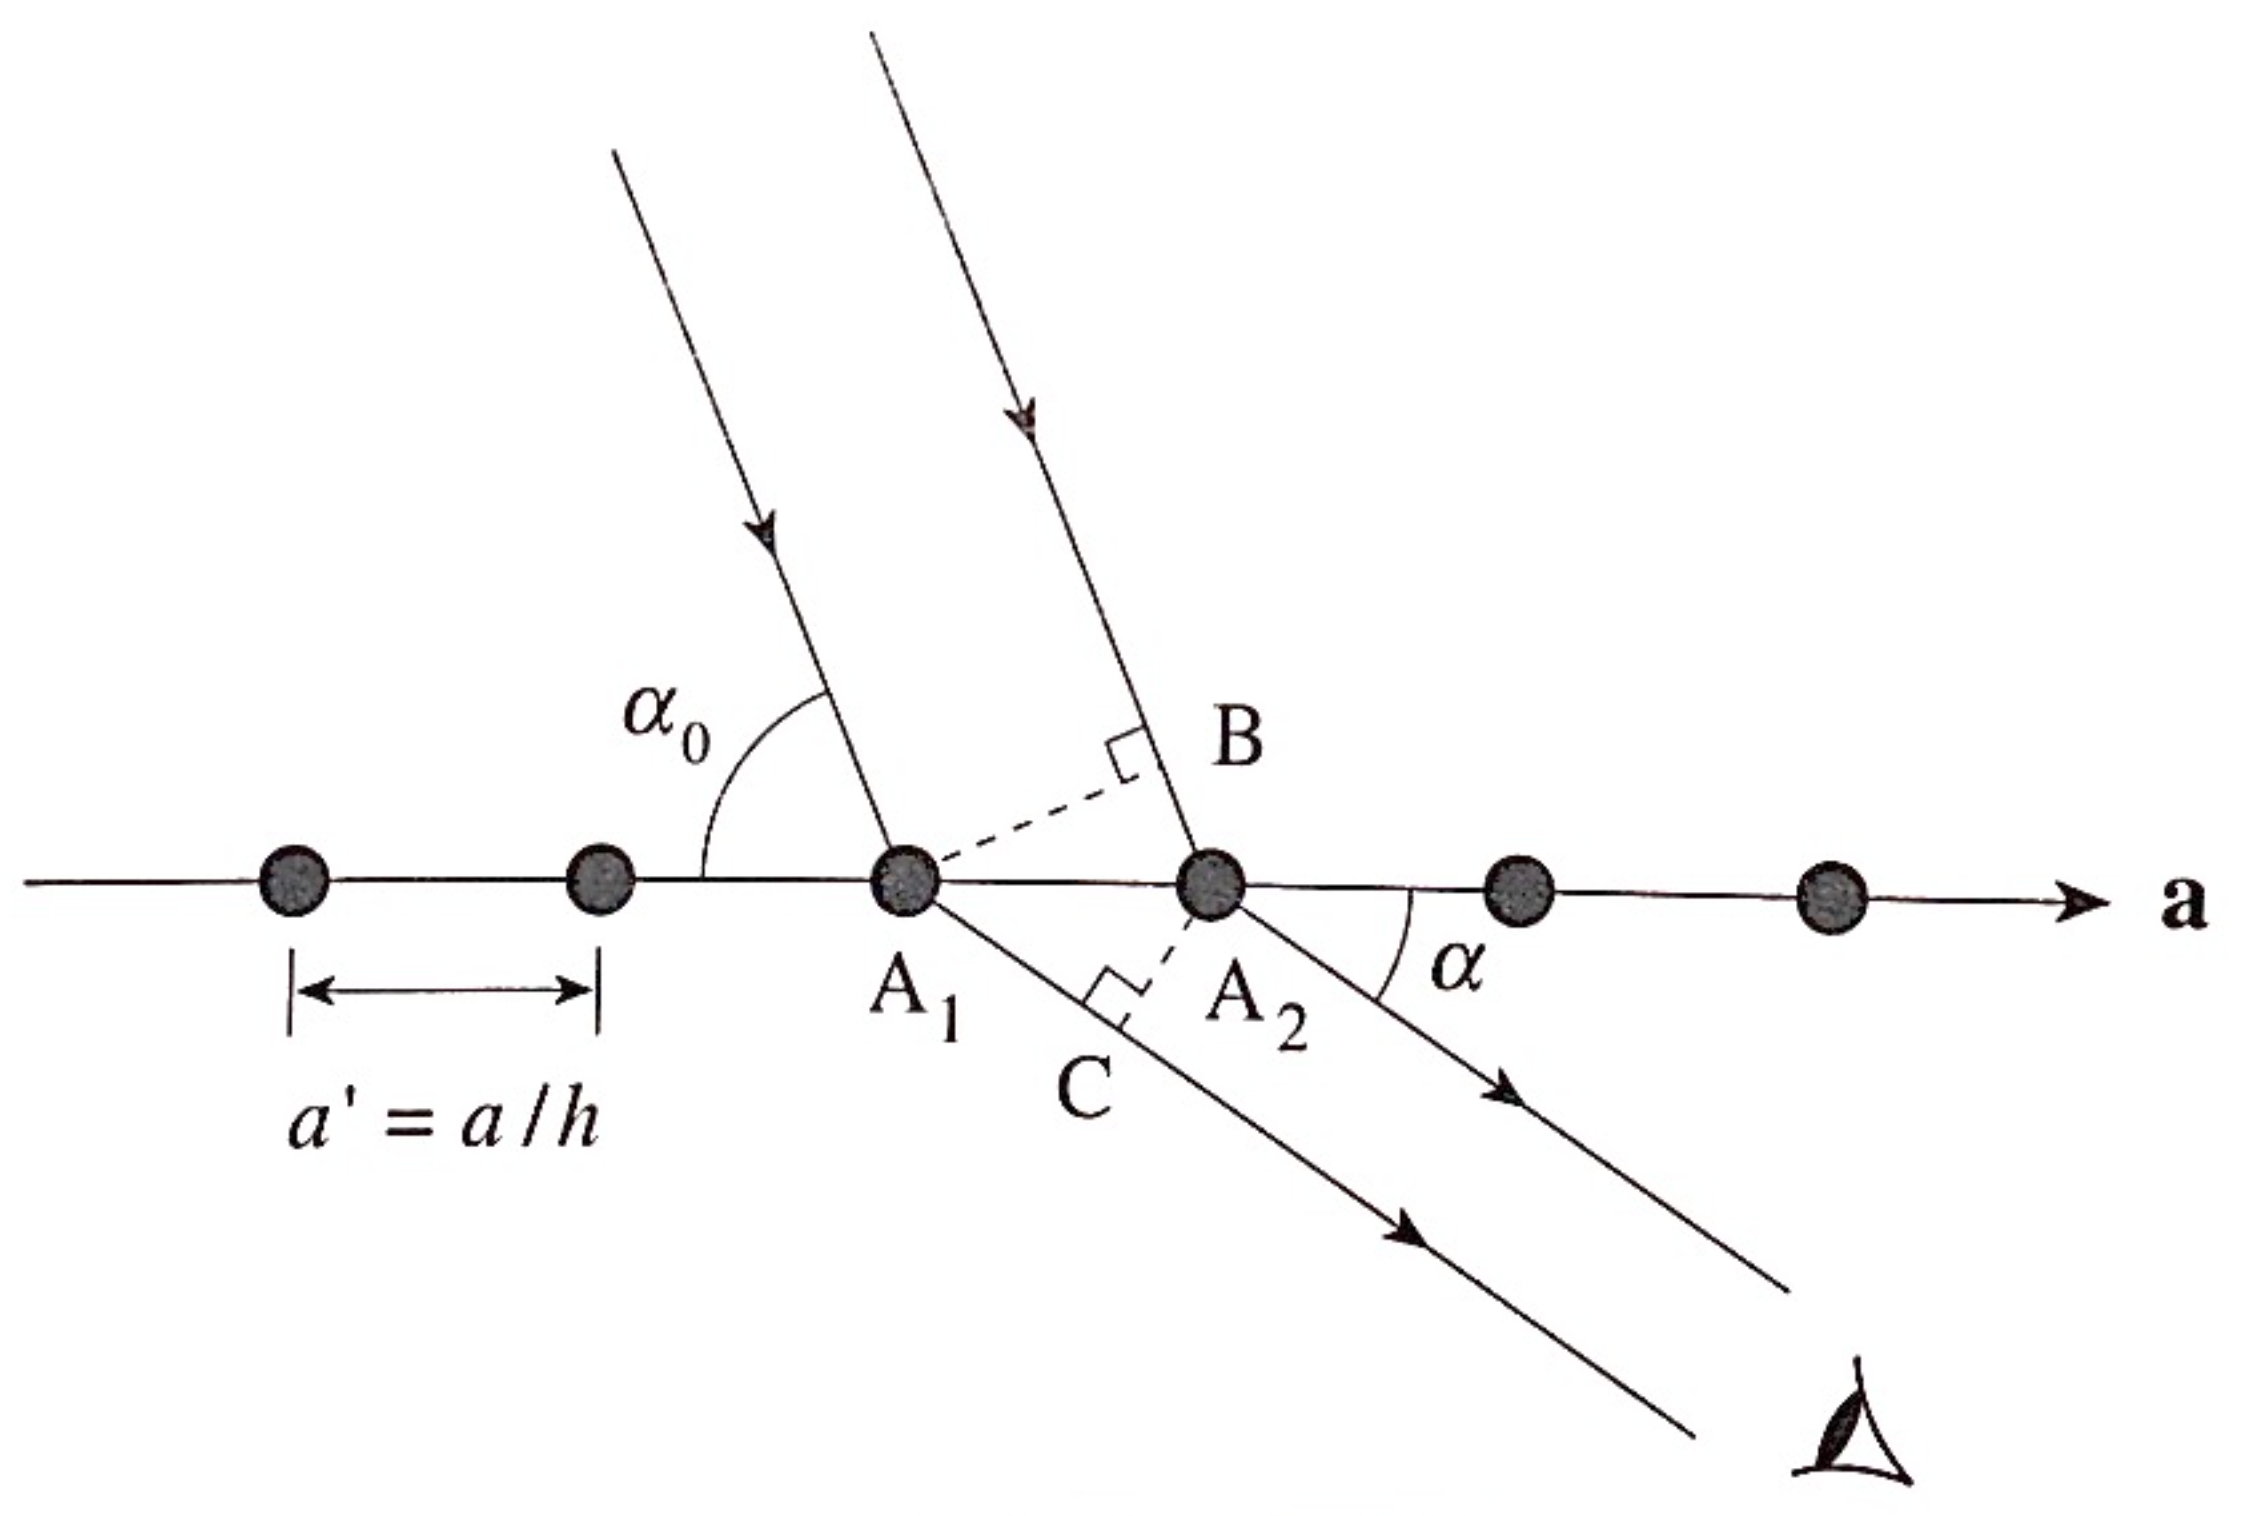
\includegraphics[width=0.45\linewidth]{../ExtFiles/vonLaueDerivation.png}
        \caption{Deriving the von Laue equations.}
        \label{fig:vonLaueDerivation}
    \end{figure}
    \begin{itemize}
        \item An X-ray diffraction pattern is a collection of spots of varying intensity.
        \begin{itemize}
            \item The arrangement of the spots provides a great deal of information on the crystal structure, as we will soon see.
        \end{itemize}
        \item We define
        \begin{equation*}
            \Delta = \overline{\text{A}_1\text{C}}-\overline{\text{A}_2\text{B}}
        \end{equation*}
        \begin{itemize}
            \item Imagine two parallel rays of light incident on points $\text{A}_1$ and $\text{A}_2$ in a crystal lattice.
            \item $\overline{\text{A}_1\text{C}}$ is the distance that the bottom beam travels after being scattered at $\text{A}_1$ and before the top beam is scattered at $\text{A}_2$.
            \item Symmetrically, $\overline{\text{A}_2\text{B}}$ is the distance that the top beam travels after the bottom beam is scattered at $\text{A}_2$ and before being scattered at $\text{A}_2$.
            \item Either way, $\Delta$ represents a kind of phase offset that occurs upon scattering. Say, for instance, that the two waves are in phase before scattering. Then from the perspective of the top wave, the bottom wave gets offset by $\Delta$ relative to it during the scattering process, and vice versa from the perspective of the bottom wave.
        \end{itemize}
        \item If the distance $\Delta$ is equal to an integral multiple of the wavelength of the X-ray radiation, the two diffracted beams will interfere constructively. Mathematically, since
        \begin{align*}
            \overline{\text{A}_1\text{C}} &= a'\cos\alpha&
            \overline{\text{A}_2\text{B}} &= a'\cos\alpha_0
        \end{align*}
        as we may readily read from Figure \ref{fig:vonLaueDerivation}, we require
        \begin{align*}
            n\lambda &= \Delta\\
            &= \overline{\text{A}_1\text{C}}-\overline{\text{A}_2\text{B}}\\
            &= a'(\cos\alpha-\cos\alpha_0)\\
            nh\lambda &= a(\cos\alpha-\cos\alpha_0)
        \end{align*}
    \end{itemize}
    \item \textbf{First-order reflection}: A diffraction spot that corresponds to $n=1$ in the above equation.
    \item \textbf{Second-order reflection}: A diffraction spot that corresponds to $n=2$ in the above equation.
    \item \textbf{$\bm{n}^\textbf{th}$-order reflection}: A diffraction spot that corresponds to $n$ in the above equation.
    \item \textbf{von Laue equations}: The following three equations, which relate the quantities involved in a first-order reflection. \emph{Given by}
    \begin{align*}
        a(\cos\alpha-\cos\alpha_0) &= h\lambda&
        b(\cos\beta-\cos\beta_0) &= k\lambda&
        c(\cos\gamma-\cos\gamma_0) &= l\lambda
    \end{align*}
    where $\alpha_0,\beta_0,\gamma_0$ are the angles of incidence of the X-ray radiation with respect to the \textbf{a}, \textbf{b}, and \textbf{c} axes of the crystal, respectively, and $\alpha$, $\beta$, and $\gamma$ are the corresponding diffraction angles.
    \item An example of how to use the von Laue equations.
    \begin{itemize}
        \item Consider the diffraction pattern obtained when an X-ray beam is directed at a crystal whose unit cell is primitive cubic.
        \item Orient the crystal such that the incident X-rays are perpendicular to the \textbf{a} axis of the crystal.
        \item Then the relevant von Laue equation reduces to $a\cos\alpha=h\lambda$.
        \item It follows that discrete angles will yield discrete spots?
    \end{itemize}
    \item A more general situation.
    \begin{itemize}
        \item For an arbitrary $hkl$ plane, the direction of diffraction with respect to the \textbf{a} axis is the same as that for the $h00$ planes. But there is also diffraction with respect to the \textbf{b} and \textbf{c} axes.
        \item The diffraction spots from an $hkl$ plane (with fixed $h$) will lie along the surface of a cone that makes an angle $\alpha$ with respect to the \textbf{a} axis of the crystal.
    \end{itemize}
    \item The Bragg diffraction.
    \begin{itemize}
        \item We have
        \begin{equation*}
            \lambda=2\left( \frac{d}{n} \right)\sin\theta
        \end{equation*}
        where $\theta$ is the angle of incidence (and reflection) of the X-rays with respect to the lattice plane, $\lambda$ is the wavelength of the X-ray radiation, and $n=1,2,\dots$ is the order of the reflection.
        \item $d$ in terms of the Miller indices for a cubic unit cell gives
        \begin{equation*}
            \sin^2\theta = \frac{n^2\lambda^2}{4a^2}(h^2+k^2+l^2)
        \end{equation*}
        \item Tian will not go through the details, but there will be a homework problem in which we will explore this.
    \end{itemize}
    \item Rotating the sample vs. rotating the incident beam in an X-ray diffraction experiment.
    \begin{itemize}
        \item In most cases, we fix the incident beam orientation and rotate the sample on the sample stage.
    \end{itemize}
    \item Midterms back today or tmw.
    \item The grade distribution in the course.
    \begin{itemize}
        \item A or A- is typically 65-70\%.
    \end{itemize}
\end{itemize}




\end{document}